% !TEX program = xelatex
\documentclass[fontset=windows,12pt,a4paper]{ctexart}
\usepackage[a4paper,margin=2.5cm,headheight=15pt]{geometry}
\usepackage{amsmath,amssymb,booktabs,array,graphicx,float,xcolor,listings,fancyhdr}
\usepackage[hidelinks,unicode]{hyperref}
\IfFontExistsTF{Times New Roman}{\setmainfont{Times New Roman}}{}
\IfFontExistsTF{Consolas}{\setmonofont{Consolas}}{}
\linespread{1.22}
\setlength{\parindent}{2em}
\setlength{\parskip}{0.15em}
\ctexset{section={number=\arabic{section},format=\large\heiti\bfseries,
  beforeskip=1.1em,afterskip=0.5em},subsection={number=\arabic{section}.\arabic{subsection},
  format=\normalsize\heiti\bfseries,beforeskip=0.7em,afterskip=0.3em}}
\pagestyle{fancy}
\fancyhf{}
\fancyhead[C]{\small 用电负荷预测与储能调度优化}
\fancyfoot[C]{\small\thepage}
\renewcommand{\headrulewidth}{0.4pt}
\renewcommand{\arraystretch}{1.16}
\setlength{\textfloatsep}{0.8em}
\setlength{\intextsep}{0.8em}
\setlength{\abovecaptionskip}{0.4em}
\setlength{\belowcaptionskip}{0.3em}
\lstset{basicstyle=\ttfamily\footnotesize,backgroundcolor=\color{black!3},
  frame=single,rulecolor=\color{black!20},breaklines=true,columns=fullflexible,
  keepspaces=true,showstringspaces=false,aboveskip=0.6em,belowskip=0.6em}
\hypersetup{pdftitle={家庭用电负荷预测与分时电价下的储能调度},
  pdfsubject={模型、回测与可执行性分析}}
\begin{document}
\begin{center}
{\LARGE\heiti\bfseries 家庭用电负荷预测与\par 分时电价下的储能调度}\par
\vspace{0.5em}
{\large 模型、回测与可执行性分析}\par
\vspace{0.4em}
{\small 项目报告}
\end{center}
\begin{center}{\heiti\bfseries 摘\quad 要}\end{center}
针对家庭储能的日前充放电安排，本文以公开家庭用电记录为输入，构建负荷预测、混合整数线性规划和真实负荷回测相衔接的实验流程。采用前一日同小时功率预测次日负荷，在假设分时电价和电池参数下比较无储能、固定规则与优化调度三种策略。2010 年 1 月 4 日至 10 日共 168 小时的预测平均绝对误差为 0.701245 kW，均方根误差为 0.991260 kW。默认 5 kWh 情景的七日日前优化均求得最优解，但仅两日满足三种策略共同可执行，覆盖率为 28.57\%。在这两日，优化策略购电费用为 50.050614 元，比无储能减少 7.0747\%。该结果属于事后筛选有效日期的条件比较，不能代表全周收益。实验表明，预测条件下的最优性需要与真实负荷下的可执行性分别检验；当前结果主要用于验证流程和识别预测误差对调度的影响。

\vspace{0.5em}
\noindent\textbf{关键词：}家庭负荷预测；储能调度；混合整数线性规划；回测；可执行性

\section{研究问题与实验思路}
分时电价为低价时段充电、高价时段放电提供了费用优化空间，但日前计划依赖尚未发生的负荷。若预测偏高，放电计划可能超过实际用电需求；在不允许向电网售电的设定下，费用较低的计划也可能无法执行。因此，本项目同时考察预测误差、计划约束和实际购电费用，避免只用优化目标值评价方案。

实验按日独立运行：先清洗历史分钟数据并聚合到小时，再预测目标日 24 小时负荷，分别生成三种策略的计划，最后冻结充放电功率，用目标日真实负荷回测。目标日真实观测只用于评价，不参与计划生成。研究对象是一户家庭的一段历史记录，电价和电池为假设情景，结论适用范围据此限定。

\section{数据、预测与实验设定}
\subsection{数据来源与评价样本}
数据来自 UCI 的 Individual Household Electric Power Consumption 数据集\cite{uci}，使用分钟级总有功功率 \texttt{Global\_active\_power}，单位为 kW。记录按数据提供的当地钟表时间处理，不额外推断时区。选取 2010 年内首个连同前一日均具有完整原始观测的连续七日区间，即 2010 年 1 月 4 日至 10 日；选期依据为观测完整性，不使用预测误差或费用结果筛选日期。

历史输入只允许连续缺失最多 5 分钟的因果前向填补，冲突时间戳作为缺失断点。可用小时由 60 个有效分钟功率取均值，小时电量为平均功率乘以 1 h。正式评价另行要求目标日每小时都有 60 个原始有效分钟，全天共 24 小时，不用填补值替代真实观测。本次七日均满足这一条件。

\subsection{预测基线与误差指标}
采用前一日同小时负荷作为日前预测基线。设 $L_{D,h}$ 为日期 $D$、小时 $h$ 的真实平均功率，则
\begin{equation}
\widehat L_{D,h}=L_{D-1,h},\qquad h=0,\ldots,23.
\label{eq:forecast}
\end{equation}
该方法无需拟合参数，便于检查时间对齐和信息边界。对全部有效预测小时计算平均绝对误差（MAE）与均方根误差（RMSE）：
\begin{equation}
\mathrm{MAE}=\frac{1}{N}\sum_{i=1}^{N}|\widehat L_i-L_i|,
\qquad
\mathrm{RMSE}=\sqrt{\frac{1}{N}\sum_{i=1}^{N}(\widehat L_i-L_i)^2}.
\label{eq:errors}
\end{equation}
两者单位均为 kW。本次 $N=168$；费用比较使用的日期集合另由三种策略的回测有效性确定，不与预测误差样本混用。

\subsection{设备假设与参数情景}
模型假设家庭负荷不受调度影响，电池充放电效率恒定，不允许售电，不计设备投资、老化和需量费用。为避免通过日末耗尽电池获得额外费用优势，两种储能策略均要求日末电量恢复至当日初始值。各日重新使用同一初始电量，因此本实验是独立日比较，不是连续跨日控制仿真。

\begin{table}[H]
\centering\small
\caption{两组电池参数设定}
\label{tab:parameters}
\begin{tabular}{lccc}
\toprule
参数 & 符号/单位 & 默认情景 & 参数对照\\
\midrule
额定容量 & kWh & 5.0 & 3.0\\
电量下限 & $E^{\min}$/kWh & 0.5 & 0.5\\
电量上限 & $E^{\max}$/kWh & 4.5 & 2.5\\
初始及末端电量 & $E^{\mathrm{init}}$/kWh & 2.5 & 1.5\\
充、放电功率上限 & $P_c^{\max},P_d^{\max}$/kW & 2.0, 2.0 & 2.0, 2.0\\
充、放电效率 & $\eta_c,\eta_d$ & 0.95, 0.95 & 0.95, 0.95\\
\bottomrule
\end{tabular}
\end{table}
假设电价为 00:00--07:00 的 0.30 元/kWh，07:00--17:00 及 22:00--24:00 的 0.60 元/kWh，以及 17:00--22:00 的 1.00 元/kWh。以上时间区间均包含起点、不包含终点；这些价格与设备均不代表该家庭的真实资费或安装情况。

\section{调度模型与回测方法}
\subsection{混合整数线性规划}
一天划分为 24 个时段，$t=0,\ldots,23$，时长 $\Delta t=1$ h。设 $c_t,d_t,g_t$ 分别为电网侧充电、放电和购电功率，单位为 kW；$E_t$ 为时段起始电池电量，单位为 kWh；$\pi_t$ 为电价，单位为元/kWh；$z_t\in\{0,1\}$ 为充放电模式变量。日前优化最小化预测购电费用：
\begin{align}
\min\quad &\sum_{t=0}^{23}\pi_t g_t\Delta t,\label{eq:objective}\\
\text{s.t.}\quad &g_t=\widehat L_t+c_t-d_t\geq0,\quad d_t\leq\widehat L_t,\label{eq:balance}\\
&0\leq c_t\leq P_c^{\max}z_t,\quad 0\leq d_t\leq P_d^{\max}(1-z_t),\label{eq:mode}\\
&E_{t+1}=E_t+\eta_c c_t\Delta t-\frac{d_t\Delta t}{\eta_d},\label{eq:energy}\\
&E^{\min}\leq E_t\leq E^{\max}\quad(t=0,\ldots,24),\label{eq:bounds}\\
&E_0=E_{24}=E^{\mathrm{init}}.\label{eq:terminal}
\end{align}
式\eqref{eq:balance}保持功率平衡，并限制放电不超过预测负荷；式\eqref{eq:mode}禁止同一时段同时充放电；式\eqref{eq:energy}考虑双向转换损耗；式\eqref{eq:bounds}和式\eqref{eq:terminal}约束电量范围及日末恢复。模型采用 PuLP 建模、CBC 求解，单线程、单日时限 30 s。程序同时检查最优性状态及日志，并独立重算功率、电量和费用约束，绝对容差为 $10^{-6}$。

\subsection{对照策略与真实负荷回测}
无储能策略令 $c_t=d_t=0$。固定规则在 00:00--07:00 充电、17:00--22:00 放电，按照窗口内的时间顺序安排功率；循环电量同时受设备边界和预测负荷限制，并满足初末电量一致。三种策略使用同一负荷、电价与评价日期，两种储能策略使用相同电池参数。

计划确定后，保持 $c_t,d_t$ 不变，以真实负荷 $L_t$ 重新计算
\begin{equation}
g_t^{\mathrm{real}}=L_t+c_t-d_t,\qquad
C_D=\sum_{t=0}^{23}\pi_tg_t^{\mathrm{real}}\Delta t.
\label{eq:replay}
\end{equation}
回测再次检查约束；若出现 $d_t>L_t$ 等违反情况，该日策略记为不可执行，费用留空，并保存违反时刻及幅度。不通过截断原计划的放电量补救，也不将失败日视为零费用。

设三种策略共同有效的日期集合为 $\mathcal C$，费用覆盖率为 $|\mathcal C|/7$，策略 $s$ 的相对节省率按合计费用计算：
\begin{equation}
r_s=1-\frac{\sum_{D\in\mathcal C}C_{D,s}}
{\sum_{D\in\mathcal C}C_{D,\mathrm{no\ storage}}}.
\label{eq:savings}
\end{equation}
该集合由实际可执行性事后确定，可能产生选择偏差，因而费用结果必须与覆盖率共同报告。

\section{实验结果与分析}
\subsection{预测误差与调度可执行性}
168 小时预测的 MAE 为 0.701245 kW，RMSE 为 0.991260 kW。图\ref{fig:prediction}给出小时序列及误差分布，展示前日同小时基线与当日负荷的偏差。误差指标汇总所有有效小时，不能直接判断计划在放电时段是否违反约束。

\begin{figure}[H]
\centering
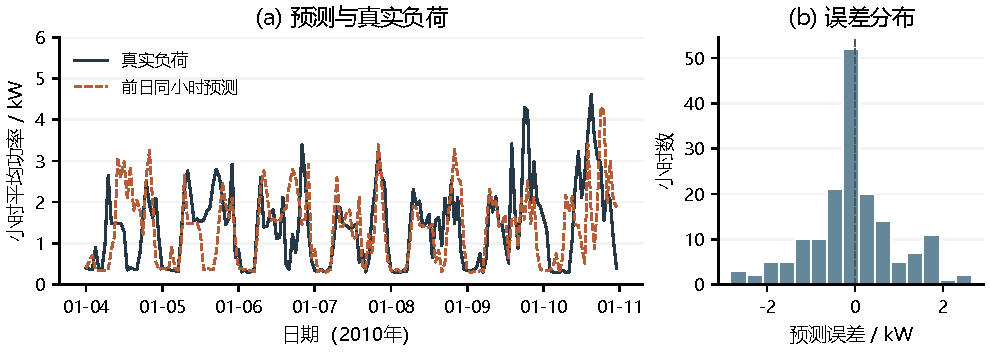
\includegraphics[width=\textwidth]{figures/prediction.pdf}
\caption{测试期小时负荷预测及误差分布。误差定义为预测值减真实值，共 168 个小时。}
\label{fig:prediction}
\end{figure}

默认 5 kWh 情景下，七日优化在预测条件下均求得最优解，独立计划检查均通过；但优化策略有五日无法通过真实负荷回测，固定规则有三日无法通过，均涉及放电超过实际负荷。这些属于回测不可执行，不是求解器未找到最优解。

\begin{table}[H]
\centering\small
\caption{默认情景逐日真实负荷回测结果}
\label{tab:validity}
\begin{tabular}{lccc}
\toprule
日期 & 无储能 & 固定规则 & 优化调度\\
\midrule
2010-01-04 & 有效 & 不可执行 & 不可执行\\
2010-01-05 & 有效 & 有效 & 有效\\
2010-01-06 & 有效 & 不可执行 & 不可执行\\
2010-01-07 & 有效 & 不可执行 & 不可执行\\
2010-01-08 & 有效 & 有效 & 不可执行\\
2010-01-09 & 有效 & 有效 & 不可执行\\
2010-01-10 & 有效 & 有效 & 有效\\
\bottomrule
\end{tabular}
\end{table}
三种策略共同有效的日期仅为 1 月 5 日和 10 日，即 $2/7=28.57\%$。这一覆盖率说明，当前预测与确定性日前优化的组合仍存在明显的执行限制。即使某日全天平均误差较小，也不能据此排除局部放电超额。

\subsection{共同有效日期的购电费用}
在相同的两日样本上，表\ref{tab:costs}比较三种策略的实际购电费用。优化调度合计比无储能减少 3.810526 元，节省率为 7.0747\%；固定规则的节省率为 4.7100\%。这些结果仅反映购电运行费用，没有包含储能投资和寿命损耗。

\begin{table}[H]
\centering\small
\caption{共同有效两日的实际购电费用比较}
\label{tab:costs}
\begin{tabular}{lrr}
\toprule
策略 & 合计费用/元 & 相对无储能节省率\\
\midrule
无储能 & 53.861140 & 0.0000\%\\
固定规则 & 51.324298 & 4.7100\%\\
优化调度 & 50.050614 & 7.0747\%\\
\bottomrule
\end{tabular}
\end{table}
两日是在回测后按三种策略均可执行筛选得到的，不能将其节省率外推到七日全周，也不能把其余日期缺失的费用补为零。本文不对全周经济收益或一般家庭储能的盈利能力作判断。

\subsection{调度案例与参数情景比较}
图\ref{fig:dispatch}给出 1 月 10 日默认情景的优化计划。电池在不同电价时段之间转移能量，电量保持在允许范围内，并在日末回到 2.5 kWh。该日通过真实负荷回测，但单日案例只能说明这一计划满足既定模型与回测条件。

\begin{figure}[H]
\centering
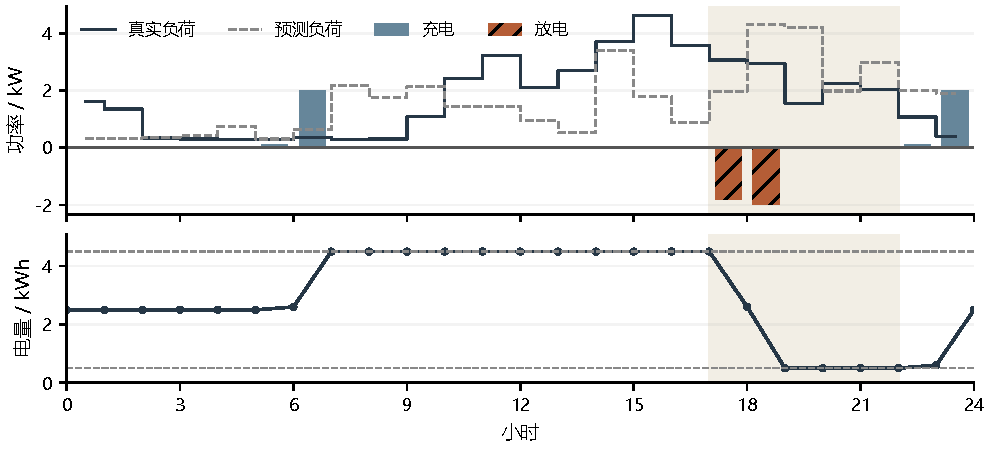
\includegraphics[width=0.94\textwidth]{figures/dispatch.pdf}
\caption{2010 年 1 月 10 日的优化调度。上图充电为正、放电为负；下图为电量轨迹及上下限。阴影表示 17:00--22:00 高价时段。}
\label{fig:dispatch}
\end{figure}

3 kWh 对照同时改变额定容量、电量上限和初始电量（表\ref{tab:parameters}），其三种策略共同有效日期为 1 月 8、9、10 日。两种情景的共同有效日期交集只有 1 月 10 日；在该日，优化购电费用由 5 kWh 情景的 26.558437 元变为 3 kWh 情景的 27.511068 元。较小的可用电量缩小了能量转移上限，但由于三项参数共同变化，该比较不构成单因素容量敏感性分析。两组各自的有效日期不同，也不能直接比较各自的费用总和来判断容量收益。

\section{讨论与结论}
本项目实现了从历史负荷处理到日前计划、真实负荷回测和失败记录的完整流程。实验中，预测条件下的最优解并不保证真实条件下可执行；放电时段的负荷高估会触发约束违反。由此，计划最优性、真实可执行性和共同样本上的费用应作为三类结果分别报告。

现有证据来自单户家庭的一周记录，费用比较只有两天共同有效，尚不足以支持普遍节费结论。前日同小时预测仅为基线，未与其他预测方法系统比较；设备和资费是假设设定，未计入投资、老化、需量费用，也未实现滚动控制、光伏、售电或真实设备接入。后续可扩大时间样本、检验更准确的预测方法，并评估滚动调度与预测不确定性约束能否提高可执行覆盖率；这些仍是待验证方向。

\begin{thebibliography}{9}
\small
\bibitem{uci} Hebrail G, Berard A. Individual Household Electric Power Consumption [DS/OL]. UCI Machine Learning Repository, 2006. DOI: \href{https://doi.org/10.24432/C58K54}{10.24432/C58K54}.
\end{thebibliography}

\section*{附录\quad 复现与实验记录}
\small
项目使用 Python 3.12，依赖版本由 \texttt{uv.lock} 锁定。报告对应实验已重新运行，环境为 Python 3.12.10、PuLP 3.3.2、CBC 2.10.3。源码、配置和依赖与仓库提交 \texttt{1333978} 一致；运行时尚未提交的文件仅为报告文档。下载原始数据后，计算可离线完成。在仓库根目录执行：
\begin{lstlisting}
uv sync --locked
uv run load-storage doctor
uv run load-storage download-data
uv run load-storage run --config configs/example.toml
uv run load-storage run --config configs/capacity3.toml
uv run pytest
\end{lstlisting}
两组实验均会保存结果后返回退出码 1，表示请求日期中存在回测失败；默认情景为五日，参数对照为四日。退出码 0 表示全部请求日期成功，2 表示运行错误。完整运行输出写入各自的 \texttt{outputs/<run\_id>/}。

随报告保留的 \texttt{docs/experiments/} 包括两组逐日策略费用与状态、168 小时预测记录、示例日优化计划及来源摘要。摘要记录原始数据 SHA-256、配置校验值、运行标识和环境版本，便于核对本文数值。原始数据约 133 MB，通过下载命令获取，不随仓库重复保存。报告采用 XeLaTeX 编译；可编辑源码和所用两张矢量图位于 \texttt{docs/report/}。
\end{document}
